\documentclass[a4paper,12pt]{article}
\usepackage[utf8]{inputenc}
\usepackage[english]{babel}
\usepackage[a4paper,top=2cm]{geometry}
\usepackage{graphicx}
\usepackage{amsmath, amssymb, amsthm}
\usepackage{listings}
\usepackage{xcolor} % Para colorir o código
\usepackage{enumitem}


\lstset{
    basicstyle=\ttfamily\small,
    keywordstyle=\color{blue},
    stringstyle=\color{red},
    commentstyle=\color{gray},
    numbers=left,
    numberstyle=\tiny\color{gray},
    breaklines=true,
    tabsize=4,
    showstringspaces=false,
}


\title{Segundo Trabalho Avaliativo de Estrutura de Dados Básica II}

\author{Raoni Silva, Pedro Galvão, Hélio Lima e Thiago Nascimento}
\date{\today}

\begin{document}

\maketitle

\noindent Turma 35M34 \\ Unidade 2

\newpage

\tableofcontents

\section{Ambiente Computacional}

Todas as implementações foram executadas e cronometradas no 
mesmo ambiente computacional, para uma comparação justa e 
adequada entre as diferentes formas de implementação das 
funções citadas no roteiro avaliativo.

O ambiente computacional consiste em uma máquina virtual no servidor pes-
soal de um dos integrantes do grupo. A máquina virtual possui dois núcleos do
processador, 2GB de memória RAM e 32GB de disco rígido à sua disposição,
rodando uma distribuição Linux conhecida como Arch Linux, com uma insta-
lação mínima, contendo somente os serviços necessários para funcionamento do
sistema operacional e o serviço de servidor SSH, para conexão remota com a
máquina.

Todas as implementações foram cronometradas utilizando os métodos apropria-
dos para cada linguagem de programação e seus respectivos tempos de execução
foram armazenados em um arquivo final, para serem analisados no presente re-
latório.

As implementações da heap foram feitas em Rust, e as árvores foram implementadas em C.
Até existiu a tentativa de criar a árvore rubro-negra em rust, mas devido a necessidade
de ter referências cíclicas, a implementação em Rust fica muito complicada.


\section{Heap}



\section{Árvore Binária}

A implementação da estrutura de árvore binária foi feita em C devido ao controle preciso de memória e à utilização eficiente de ponteiros, características essenciais dessa linguagem. 

\subsection{Definição}

Uma árvore binária é uma estrutura de dados composta por um conjunto finito de elementos, chamados de nós, sendo que o primeiro nó, denominado raiz, é o ponto inicial da árvore e o os nós da base são conhecidos como folhas. Em uma árvore binária, cada nó pode ter no máximo dois filhos, um à esquerda e outro à direita.

A árvore binária tem a propriedade de que todos os nós de uma subárvore à direita de um nó são maiores do que o valor armazenado na raiz desse nó, enquanto todos os nós de uma subárvore à esquerda de um nó são menores do que o valor armazenado na raiz desse nó. Além disso, cada subárvore, formada pelos filhos à esquerda e à direita de qualquer nó, é também uma árvore binária por si mesma. Isso torna a estrutura recursiva, em que cada nó pode ser considerado a raiz de uma nova árvore binária.

Essa organização permite operações eficientes de busca, inserção e remoção, com a garantia de que a árvore estará estruturada de forma hierárquica e balanceada.

\subsection{Estrutura}

Na implementação da árvore binária, utilizamos uma estrutura do tipo struct para representar os nós da árvore. Cada nó contém três componentes principais: um valor, representado pela chave, e dois ponteiros, um para a subárvore à esquerda e outro para a subárvore à direita. A seguir, temos a definição da estrutura:

\vspace{3mm}

\begin{lstlisting}
typedef struct arvore_t {
  int chave;
  struct arvore_t *esq;
  struct arvore_t *dir;
} arvore_t;
\end{lstlisting}

\vspace{3mm}

\subsection{Operações de Manipulação}

\subsubsection{Inserção}

Na operação de inserção em uma árvore binária, é fundamental que as propriedades da árvore sejam preservadas. Isso significa que todos os nós da subárvore à esquerda de um nó devem conter valores menores que a chave desse nó, e todos os nós da subárvore à direita devem conter valores maiores. Além disso, todo novo nó inserido na árvore sempre será uma folha, ou seja, não possuirá filhos imediatamente após sua criação.

A seguir, apresentamos o código que implementa essa operação:

\vspace{3mm}

\begin{lstlisting}
arvore_t *inserir(arvore_t *arvore, int chave) {
  if (arvore == NULL) {
    arvore = (arvore_t *)malloc(sizeof(arvore_t));
    arvore->chave = chave;
    arvore->esq = NULL;
    arvore->dir = NULL;
  } else if (chave < arvore->chave) {
    arvore->esq = inserir(arvore->esq, chave);
  } else if (chave > arvore->chave) {
    arvore->dir = inserir(arvore->dir, chave);
  }
  return arvore;
}
\end{lstlisting}

\subsubsection{Criação de Árvore a partir de uma Lista}

Para construir uma árvore binária a partir de uma lista, de forma que ela fique balanceada ou aproximadamente balanceada, foi adotada a seguinte estratégia:

\begin{enumerate}[label=\textbf{Etapa \arabic*:}]
    \item Início.
    \item Verifica se o tamanho da lista é 0.
          \begin{itemize}
              \item Se sim, retorna \texttt{NULL}.
              \item Caso contrário, chama a função \texttt{construir\_arvore}.
          \end{itemize}
    \item Calcula o índice do meio.
    \item Insere a chave central na árvore.
    \item Chama recursivamente:
          \begin{itemize}
              \item Subárvore esquerda: \texttt{construir\_arvore(chaves, inicio, meio-1, arvore)}.
              \item Subárvore direita: \texttt{construir\_arvore(chaves, meio+1, fim, arvore)}.
          \end{itemize}
    \item Retorna a árvore construída.
    \item Finaliza liberando memória.
\end{enumerate}

O código a seguir implementa essa abordagem:

\begin{lstlisting}
arvore_t *construir_arvore(int *chaves, int inicio, int fim, arvore_t *arvore) {
  if (inicio > fim) {
    return arvore;
  }
  int meio = (inicio + fim) / 2;
  arvore = inserir(arvore, chaves[meio]);
  arvore = construir_arvore(chaves, inicio, meio - 1, arvore); // Lado esquerdo
  arvore = construir_arvore(chaves, meio + 1, fim, arvore);    // Lado direito
  return arvore;
}
arvore_t *lista_p_arvore(int *chaves, int tamanho) {
  arvore_t *arvore = NULL;
  if (tamanho == 0) {
    return arvore;
  }
  arvore = construir_arvore(chaves, 0, tamanho - 1, arvore);
  return arvore;
}
\end{lstlisting}

\subsubsection{Remoção}

O processo de remoção considera três casos principais: o nó a ser removido não possui filhos, possui apenas um filho ou possui dois filhos. Quando o nó possui dois filhos, o menor elemento da subárvore direita (ou o maior da subárvore esquerda) substitui o nó removido, mantendo a organização da árvore. Para isso, utilizamos um nó auxiliar.

A seguir, apresentamos a implementação da operação de remoção:

\vspace{3mm}

\begin{lstlisting}
arvore_t *remover(arvore_t *arvore, int chave) {
  if (arvore == NULL)
    return NULL;
  if (chave < arvore->chave) {
    arvore->esq = remover(arvore->esq, chave);
  } else if (chave > arvore->chave) {
    arvore->dir = remover(arvore->dir, chave);
  } else {
    if (arvore->esq == NULL) {
      arvore_t *temp = arvore->dir;
      free(arvore);
      return temp;
    } else if (arvore->dir == NULL) {
      arvore_t *temp = arvore->esq;
      free(arvore);
      return temp;
    }
    arvore_t *rightMin = find_min(arvore->dir);
    arvore->chave = rightMin->chave;
    arvore->dir = remover(arvore->dir, rightMin->chave);
  }
  return arvore;
}
\end{lstlisting}

\subsection{Operações de Consulta}

\subsubsection{Busca}

Na operação de busca em uma árvore binária, o valor procurado é comparado recursivamente com a chave do nó atual, começando pela raiz. Se o valor for menor que a chave, a busca continua na subárvore à esquerda; se for maior, prossegue na subárvore à direita. Esse processo se repete até que o valor seja encontrado ou até alcançar uma folha (nó nulo), indicando que o valor não está presente na árvore.

A implementação da busca é apresentada a seguir:

\vspace{3mm}

\begin{lstlisting}
arvore_t *buscar(arvore_t *arvore, int chave) {
  if (arvore == NULL) {
    return 0;
  }
  if (chave < arvore->chave) {
    return buscar(arvore->esq, chave);
  }
  if (chave > arvore->chave) {
    return buscar(arvore->dir, chave);
  }
  if (chave == arvore->chave) {
    return arvore;
  }
  return NULL;
}
\end{lstlisting}

\subsubsection{Consulta Em Ordem}

Na consulta em ordem, os nós da árvore binária são visitados seguindo a sequência: filho da esquerda, raiz e, por fim, filho da direita. Esse tipo de travessia resulta em uma listagem dos elementos em ordem crescente, caso a árvore seja uma árvore binária de busca.

\begin{lstlisting}
void mostrarEmOrdem(arvore_t *arvore) {
  if (arvore != NULL) {
    mostrarEmOrdem(arvore->esq);
    printf("  %d", arvore->chave);
    mostrarEmOrdem(arvore->dir);
  }
}
\end{lstlisting}

\subsubsection{Consulta Em Pré Ordem}

Na consulta em pré-ordem, os nós são visitados na seguinte sequência: raiz, filho da esquerda e filho da direita. Esse método é frequentemente utilizado para gerar uma cópia da árvore ou para fins de visualização estrutural.

\begin{lstlisting}
void mostrarEmOrdem(arvore_t *arvore) {
  if (arvore != NULL) {
    mostrarEmOrdem(arvore->esq);
    printf("  %d", arvore->chave);
    mostrarEmOrdem(arvore->dir);
  }
}
\end{lstlisting}

\subsubsection{Consulta Em Pós Ordem}

Na consulta em pós-ordem, a visita aos nós segue a ordem: filho da esquerda, filho da direita e, por último, a raiz. Esse tipo de travessia é útil em operações que envolvem a remoção ou processamento dos nós em uma sequência de base para topo (por exemplo, liberar memória ou avaliar expressões em árvores de sintaxe).

\begin{lstlisting}
void mostrarPosOrdem(arvore_t *arvore) {
  if (arvore != NULL) {
    mostrarPosOrdem(arvore->esq);
    mostrarPosOrdem(arvore->dir);
    printf("  %d", arvore->chave);
  }
}
\end{lstlisting}

\subsubsection{Consulta Em Nível}

Para realizar uma consulta em nível, ou seja, visitar os nós da árvore da raiz até as folhas, seguindo uma ordem horizontal (nível por nível), é possível utilizar ferramentas gráficas que convertem arquivos no formato DOT para imagens, como arquivos PNG. Esse proceso permite obter a seguinte visualização da árvore:

\begin{figure}[h!]
    \centering
    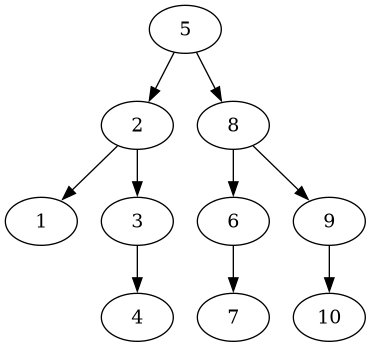
\includegraphics[width=0.3\textwidth]{imagens/arvore_de_busca0.png}
    \caption{}
    \label{fig:exemplo}
\end{figure}


\section{Árvore AVL}

Esta seção apresenta a implementação completa de uma Árvore AVL, esta a seguir, desenvolvida na linguagem C,
incluindo suas principais operações: inserção, remoção, balanceamento, busca. 
Além disso, para fins de visualização, também foi implementada uma funcionalidade de exportação para formato DOT.
A Árvore AVL é uma árvore binária de busca auto-balanceada que garante operações eficientes, como inserções e buscas, mantendo a complexidade \(O(\log n)\).

\vspace{3mm}

\subsection{Estrutura de Dados}

\vspace{3mm}

A estrutura de dados da Árvore AVL (\texttt{arvore\_avl}) é definida com os seguintes atributos:

\begin{lstlisting}
typedef struct arvore_avl {
    int valor;                // Valor armazenado no nó
    int altura_esq;           // Altura da subárvore esquerda
    int altura_dir;           // Altura da subárvore direita
    struct arvore_avl *esq;   // Ponteiro para o filho esquerdo
    struct arvore_avl *dir;   // Ponteiro para o filho direito
} arvore_avl;
\end{lstlisting}

O campo \texttt{valor} armazena o dado do nó, enquanto \texttt{altura\_esq} e \texttt{altura\_dir} mantêm a altura de cada subárvore. 
Isso facilita o balanceamento da árvore, que é realizado após cada inserção ou remoção.

\vspace{3mm}

\subsection{Funções Principais da Árvore AVL}

\vspace{3mm}

\subsubsection{Cálculo da Altura}

\vspace{3mm}

A função \texttt{calcular\_altura} retorna a altura da subárvore. Caso o nó seja nulo (\texttt{NULL}), a altura será considerada 0. 
Este cálculo é essencial para determinar se a árvore precisa de balanceamento.

\begin{lstlisting}
int calcular_altura(arvore_avl *arv) {
    if (arv == NULL) {
        return 0;
    }
    int altura_esq = calcular_altura(arv->esq);
    int altura_dir = calcular_altura(arv->dir);
    return (altura_esq > altura_dir ? altura_esq : altura_dir) + 1;
}
\end{lstlisting}

\vspace{3mm}

\subsubsection{Criação de um Novo Nó}

\vspace{3mm}

A função \texttt{criar\_novo\_no} aloca memória para um novo nó da árvore e inicializa seus campos.

\begin{lstlisting}
arvore_avl *criar_novo_no(int valor) {
    arvore_avl *novo_no = (arvore_avl *)malloc(sizeof(arvore_avl));
    if (novo_no == NULL) {
        fprintf(stderr, "Erro ao alocar memória para o nó.\n");
        exit(1);
    }
    novo_no->valor = valor;
    novo_no->altura_esq = 0;
    novo_no->altura_dir = 0;
    novo_no->esq = NULL;
    novo_no->dir = NULL;
    return novo_no;
}
\end{lstlisting}

\vspace{3mm}

\subsubsection{Rotações de Balanceamento}

\vspace{3mm}

O balanceamento da Árvore AVL é garantido por meio de rotações,
que reorganizam os nós para manter a diferença de altura entre as subárvores esquerda e direita dentro do limite de 1.

\paragraph{Rotação à Esquerda}  
A rotação à esquerda reorganiza os nós em torno do filho direito do nó desbalanceado.

\begin{lstlisting}
arvore_avl *rotacao_esquerda(arvore_avl *raiz) {
    if (raiz == NULL || raiz->dir == NULL) {
        return raiz;
    }
      
    arvore_avl *novo_raiz = raiz->dir;
    arvore_avl *subarvore_dir = novo_raiz->esq;
      
    novo_raiz->esq = raiz;
    raiz->dir = subarvore_dir;
      
    raiz->altura_esq = calcular_altura(raiz->esq);
    raiz->altura_dir = calcular_altura(raiz->dir);
      
    novo_raiz->altura_esq = calcular_altura(novo_raiz->esq);
    novo_raiz->altura_dir = calcular_altura(novo_raiz->dir);
      
    return novo_raiz;
}
\end{lstlisting}

\paragraph{Rotação à Direita}  
A rotação à direita é o análogo da rotação à esquerda, mas reorganiza os nós em torno do filho esquerdo.

\begin{lstlisting}
arvore_avl *rotacao_direita(arvore_avl *raiz) {
    if (raiz == NULL || raiz->esq == NULL) {
        return raiz;
    }
      
    arvore_avl *novo_raiz = raiz->esq;
    arvore_avl *subarvore_esq = novo_raiz->dir;
      
    novo_raiz->dir = raiz;
    raiz->esq = subarvore_esq;
      
    raiz->altura_esq = calcular_altura(raiz->esq);
    raiz->altura_dir = calcular_altura(raiz->dir);
      
    novo_raiz->altura_esq = calcular_altura(novo_raiz->esq);
    novo_raiz->altura_dir = calcular_altura(novo_raiz->dir);
      
    return novo_raiz;
}
\end{lstlisting}

\vspace{3mm}

\subsubsection{Inserção de um Nó}

\vspace{3mm}

A função \texttt{inserir\_no} insere um valor na árvore de maneira recursiva. Após cada inserção, a árvore é balanceada.

\begin{lstlisting}
arvore_avl *inserir_no(arvore_avl *raiz, int valor) {
    arvore_avl *novo_no;
      
    if (raiz == NULL) {
        return criar_novo_no(valor);
    }
      
    if (valor < raiz->valor) {
        raiz->esq = inserir_no(raiz->esq, valor); 
    } else if (valor > raiz->valor) {
        raiz->dir = inserir_no(raiz->dir, valor); 
    }
      
    raiz->altura_esq = calcular_altura(raiz->esq);
    raiz->altura_dir = calcular_altura(raiz->dir);
      
      
    raiz = balancear_arvore(raiz);
    return raiz;
}
\end{lstlisting}

\vspace{3mm}

\subsubsection{Remoção de um Nó}

\vspace{3mm}

A função \texttt{remover\_no} remove um valor da árvore e a rebalanceia, quando necessário.

\begin{lstlisting}
arvore_avl *remover_no(arvore_avl *raiz, int valor) {
    if (raiz == NULL) {
        return NULL;
    }
      
    if (valor < raiz->valor) {
        raiz->esq = remover_no(raiz->esq, valor);
    } else if (valor > raiz->valor) {
        raiz->dir = remover_no(raiz->dir, valor);
    } else {
        if (raiz->esq == NULL && raiz->dir == NULL) {
        free(raiz);
        return NULL;
        } else if (raiz->esq == NULL) {
        arvore_avl *aux = raiz->dir;
        free(raiz);
        return aux;
        } else if (raiz->dir == NULL) {
        arvore_avl *aux = raiz->esq;
        free(raiz);
        return aux;
        } else {
        arvore_avl *aux = raiz->dir;
        while (aux->esq != NULL) {
            aux = aux->esq;
        }
        raiz->valor = aux->valor;
        raiz->dir = remover_no(raiz->dir, aux->valor);
        }
    }
      
    raiz->altura_esq = calcular_altura(raiz->esq);
    raiz->altura_dir = calcular_altura(raiz->dir);
  
    return balancear_arvore(raiz);
}
\end{lstlisting}

\vspace{3mm}

\subsubsection{Busca em uma Árvore AVL}

\vspace{3mm}

A função \texttt{buscar} localiza um valor na árvore. Caso o valor não seja encontrado, retorna \texttt{NULL}.

\begin{lstlisting}
arvore_avl *buscar(arvore_avl *raiz, int valor) {

    if (raiz == NULL) {
      return 0;
    }
  
    if (valor < raiz->valor) {
      return buscar(raiz->esq, valor);
    }
  
    if (valor > raiz->valor) {
      return buscar(raiz->dir, valor);
    }
  
    if (valor == raiz->valor) {
      return raiz;
    }
    return NULL;
}
\end{lstlisting}

\subsubsection{Exportação para DOT}

A função \texttt{exportar\_para\_dot}, em conjunto com a função \texttt{gerar\_dot}, gera um arquivo no formato DOT, possibilitando a visualização da árvore em ferramentas gráficas.
Embora essa funcionalidade não seja uma característica intrínseca de uma Árvore AVL,
foi incluída neste código para tornar sua análise mais acessível e intuitiva, facilitando a compreensão de sua estrutura e funcionamento.

\begin{lstlisting}
void exportar_para_dot(arvore_avl *raiz, const char *nome_arquivo) {
    FILE *arquivo = fopen(nome_arquivo, "w");
    if (arquivo == NULL) {
        fprintf(stderr, "Erro ao abrir o arquivo %s\n", nome_arquivo);
        exit(1);
    }

    fprintf(arquivo, "digraph G {\n");
    gerar_dot(arquivo, raiz);
    fprintf(arquivo, "}\n");
    fclose(arquivo);
}
\end{lstlisting}

\vspace{3mm}

\subsection{Conclusão sobre a arvore AVL}

\vspace{3mm}

A Árvore AVL é uma estrutura de dados solida e eficiente para manipulação de informações. 
Ela assegura que as operações de busca, inserção e remoção sejam realizadas em tempo 
O(logn), graças ao balanceamento automático proporcionado pelos cálculos de altura e rotações. 
Essa característica permite que a árvore permaneça equilibrada, independentemente da ordem em que os nós são inseridos ou removidos. 
Por sua eficiência, as Árvores AVL têm ampla aplicação em sistemas que exigem alto desempenho,
como bancos de dados, sistemas de arquivos e em outras diversas áreas da computação.
\section{conclusão}

Neste relatório, exploramos os principais algoritmos de inserção, remoção e busca, 
que garantem a manutenção da balanceamento da árvore, permitindo operações eficientes. 
A implementação da árvore B, com suas operações de redistribuição e concatenação durante a 
remoção, oferece um excelente compromisso entre complexidade e desempenho, tornando-a uma 
ferramenta fundamental para o gerenciamento de dados em larga escala.


\end{document}